\documentclass{amia_summit_2018}
\usepackage{graphicx}
\usepackage[labelfont=bf]{caption}
\usepackage[superscript,nomove]{cite}
\usepackage{color}
\usepackage{multirow}
\renewcommand*{\thefootnote}{\fnsymbol{footnote}}

\begin{document}

\title{Predicting Success of Motivational Interviews with Recurrent Neural Network and Probabilistic Model for Patient-Provider Communication Sequences}

\author{Mehedi Hasan, BS$^{1}$\footnote[1]{Authors provided equal contribution. \label{footnote1}}, Alexander Kotov, PhD$^{1}$\textsuperscript{\ref{footnote1}}, April Idalski Carcone, PhD$^{2}$, Ming Dong, PhD$^{1}$, Sylvie Naar, PhD$^{2}$}

\institutes{
$^1$Department of Computer Science,  
$^2$Department of Family Medicine and Public Health Sciences, School of Medicine, Wayne State University, Detroit, Michigan\\
}

\maketitle

\noindent{\bf Abstract}
\textit{The problem of analyzing temporally ordered observation sequences to make predictions related to the outcome of the processes that generated these sequences arises in many domains of healthcare informatics. In this paper, we focus on patient-provider communication sequences in the context of clinical interviews and propose Recurrent Neural Network (RNN) with two baseline methods Markov chain and Hidden Markov Model (HMM), for predicting the likelihood of eliciting a particular type of patient behavioral response based on an observed sequence of patient-provider exchanges. Our method achieved 70.38\%, 60.67\%, 86.77\% F1-score for under-sampled sequences and 77.75\%, 75.20\%, 83.81\% F1-score for over-sampled sequences in predicting the outcome of motivational interviews with obese adolescents using Markov Chain, HMM, and RNN, respectively. The proposed method can be used to automatically identify the most effective communication strategies in motivational interviews, which significantly decreases the effort required to develop effective interventions to address many public health conditions.}

\section*{Introduction}
Data in the form of temporally ordered sequences of discrete or continuous observations (e.g., symbolic sequences such as notes in patient EHR, diagnostic codes, protein or DNA sequences or continuous time series, such as ECG measurements) arise in various domains of health informatics. Sequence classification methods are utilized for classifying temporally ordered sequences. Sequence classification has a broad range of real word applications from genomics and health informatics to finance and anomaly detection \cite{yakhnenko2005discriminatively, wei2006semi, lane1999temporal}. In genomics research, sequence classification is widely used to classify protein and text sequence data and detect the function of new proteins. In health informatics, ECG measurements are considered as multi-dimensional time series and are used to classify individuals as healthy or having a heart disease. Sequence classification is also used for anomaly detection such as abnormal access to systems and malware.

%Sequence classification has a broad range of real word applications from genomics and health informatics to finance and anomaly detection. In genomics research, sequence classification is widely used to classify protein and text sequence data \cite{yakhnenko2005discriminatively} and detect the function of new proteins \cite{deshpande2002evaluation}. In health informatics, ECG measurements are considered as multi-dimensional time series and are used to classify individuals as healthy or having a heart disease \cite{wei2006semi}. Sequence classification is also used for anomaly detection such as abnormal access to systems \cite{lane1999temporal} and malware \cite{drew2017polymorphic}.

In general, there are three categories of classification methods for temporally ordered sequences, e.g.: feature-based, distance metric-based and model-based method. Feature-based classification methods transform a sequence into a feature vector and apply a standard supervised learning algorithm, such as support vector machine \cite{leslie2004fast} or decision tree \cite{chuzhanova1998feature}. 
%Shapelet \cite{ye2009time} and pattern \cite{kudenko1998feature, lesh1999mining} based techniques as well as hierarchical approaches \cite{nallam2016effective} have been proposed instead of standard classifiers as well. 
Distance-based methods measure the similarity between sequences of behavior codes to determine the quality of classification. The most commonly used distance function is euclidian distance with Dynamic Time Wrapping \cite{keogh2000scaling} used for more flexible matching in time series data.  
%The most commonly used distance function is Euclidian distance \cite{keogh2003need} with Dynamic Time Wrapping \cite{keogh2000scaling} used for more flexible matching in time series data. 
The order of observations in a sequence is challenging to model using feature-based methods because the traditional bag-of-words representation of features does not account for the order of observation. At the same time, distance-based methods are more appropriate for time series data. Model-based classification methods involve building a model based on the dataset. In other words, information is learned from the dataset, and used as a ``model'' to classify sequences.  

%This makes sequence classification a more challenging task than traditional classification.  

One of the model-based classification methods is probabilistic model, which creates a model of behavioral code sequences, such as Markov Chain (MC) and Hidden Markov Model \cite{rabiner1989tutorial} (HMM). Markov models have limitations when applied to sequence classification because they cannot preserve long-term dependencies in sequences. Similarly, the hidden states of HMMs follow a first-order Markov chain and can select only one hidden state at each time step. Therefore, Markov chain and HMMs are usually used for passing one or two preceding step(s) among sequence steps\cite{kundu1988recognition}. On the other hand, Recurrent Neural Networks (RNNs) have no such limitations in preserving long-term dependencies among sequence steps due to their unlimited memory. It was shown that RNNs are very effective in a wide range of sequence modeling problems with temporal data\cite{nion2013handwritten, lipton2015learning, choi2016doctor}. A variant of RNN called Long Short-Term Memory was proposed \cite{graves2013speech} which solved the vanishing gradient problem \cite{bengio1993problem} of traditional RNN. LSTM showed excellent performance in several domains, including speech recognition \cite{graves2013speech}, handwriting recognition \cite{nion2013handwritten} and health informatics \cite{lipton2015learning, choi2016doctor}. In Lipton et. al.\cite{lipton2015learning}, LSTM was used as a multilabel classification model to recognize patterns in multivariate time series of clinical measurements such as body temperature, heart rate, blood pressure, etc. LSTM was also effectively used for designing a model, called Doctor AI \cite{choi2016doctor}, for predicting the diagnosis and medication categories of a subsequent visit. A further simplification and improvement of the LSTM model, called the Gated Recurrent Unit\cite{chung2014empirical} (GRU), was later proposed. These variants show markedly improved performance among all RNN variants and as such, this work focuses on these variants of RNN specifically.       

Childhood obesity is a serious public health concern in the United States and worldwide. Recent estimates indicate that approximately one-third (31.8\%) of US children age 2-19 years are overweight and 16.9\% are obese \cite{ogden2012prevalence}. Adolescents who are obese likely continue to be obese in adulthood and have a greater risk of heart disease, type 2 diabetes, stroke, cancer, and osteoarthritis \cite{general2010surgeon}. One approach to effective obesity intervention is Motivational Interviewing, an evidence-based counseling technique to increase intrinsic motivation and self-efficacy for health-related behavior change. The goal of MI is to encourage patients to explore their own desires, ability, reasons, need for and commitment to the targeted behavior change. These statements, referred to as ``change talk'' or CHT, consistently predict actual behavior change\cite{apodaca2009mechanisms} that can be sustained for as long as 34 months\cite{walker2011influence} after an interview. However, the ability of counselors to consistently elicit this type of patient communication requires knowledge of effective communication strategies for a variety of patients, which can only be obtained through analysis of a large number of annotated interviews. Since manual examination and sequential pattern analysis of transcripts is a very time-consuming process, tailoring of MI interventions to particular populations can take years. Therefore, there is a need for informatics-based methods to facilitate the development of effective MI-based interventions, in general, and theoretically-grounded computational models to explore the mechanisms of MI's efficacy, in particular.  

%This work is the next step in a series of experiments to develop the [informatics based methods described above]. 
In our previous work \cite{kotov2015interpretable, hasan2016study}, we explored several machine learning methods for automatic annotation of clinical interview fragments with a specialized codebook containing a large number of patient and provider behavior codes \cite{carcone2013provider}. In this paper, we test the applicability of state-of-the-art models for the classification of patient-provider communication sequences in the context of clinical interviews. Specifically, we focus on the transcripts of Motivational Interviews (MI) with obese adolescents and their caregivers.
We propose Recurrent Neural Networks with two baseline probabilistic methods, MC and HMM, to identify patient-provider communication sequences that are likely to elicit the desired patient behavioral response (i.e. change talk or commitment language) and to dynamically estimate the likelihood of observing this desired response at any point during a clinical interview based on all coded previous patient-provider communication exchanges in the same interview. While there have been some previous qualitative studies of patient-provider dialog in a clinical setting \cite{eide2004physician}, there have been no previous work on computational modeling of annotated patient-provider communication (PPC) exchanges and predicting the desired patient behavior in a context of motivational interviews.   

\section*{Methods}
\subsection*{\textit{Data collection}}
The experimental dataset for this work was constructed from the transcripts of 129 motivational interviews, which include a total of 50,239 segmented and annotated utterances. Each transcript consists of an MI interview session involving counselor, adolescent, and caregiver. The utterances were annotated based on MYSCOPE codebook \cite{carcone2013provider}, which are grouped into client codes (adolescent and caregiver) group and counselor codes group. Utterances were divided into successful and unsuccessful communication sequences. Successful communication sequences result in positive change talk and commitment language statements by an adolescent or caregiver, while unsuccessful sequences are the ones that result in negative change talk or commitment language and the sequences, in which no change talk or commitment language statements occur. Out of 5143 observed sequences, 4225 were positive and 918 were negative. Here, the successful sequences had an average length of 9.79 while that of unsuccessful sequences was 9.65. For each of the probabilistic models (Markov chain and HMM), two models were trained, one model was trained using successful sequences and another one was trained using unsuccessful sequences. 

%Statistics of the experimental dataset are presented in Table~\ref{tab:data_dist}. \\
%
%\begin{table}[h]
%\centering
%\caption{Statistics of experimental dataset. Sequence length is the number of behavior codes in it.}
%\label{tab:data_dist}
%  \begin{tabular}{|l|l|l|l|l|}
%  \hline
%   \textbf{Sequence Type} & \textbf{\# of sequences}  & \textbf{Ratio} & \textbf{Average length} \\ \hline      
%Successful sequences & 4225 & 82.15\% & 9.79 \\\hline
%Unsuccessful sequences & 918 & 17.85\% & 9.65 \\\hline
%  \end{tabular}
%\end{table} 

Our data set is imbalanced and predominately composed of successful sequences with only a small percentage (17.85\%) of unsuccessful sequences. Usually, predictive accuracy misrepresents the performance of an employed algorithm for an imbalanced data. Because simply predict the majority class (successful) would provide a predictive accuracy 82.15\%. Therefore, it is important to handle imbalance data properly. Many solutions are proposed to deal with the imbalanced data sets, which can be divided into two categories: data level and algorithmic level. In this study, we utilized undersampling and oversampling methods at data processing level for balancing the adolescent obesity data set. Synthetic Minority Over Sampling Technique (SMOTE) is the most widely used method for oversampling an imbalanced dataset, in which new synthetic examples were generated from minority class \cite{chawla2002smote}. We generated synthetic examples along the borderline between minority examples and their selected nearest neighbors \cite{nguyen2011borderline}. On the other hand, the undersampling method under samples the majority class by replacing a cluster of majority samples by the cluster centroid of a K-Means algorithm.  

A fragment of an adolescent session transcript is presented in Table~\ref{tab:anno_examp}. Hence, annotation column shows the successful sequence of behavior codes from top to bottom, in particular, ($SS\rightarrow OQO\rightarrow HUPO\rightarrow OQTBN\rightarrow CHT+$) is a successful behavior sequence, where counselor starts with a structured session and gets positive change talk at the end. It was noticed that same context ``Yeah" and ``Yes'' represent different behavior codes CHT+ and HUPW, respectively. Because human brain can remember the past behaviors, and classify the current context into different behavior codes after considering their past behaviors. For this reason, we only consider those models that can capture the past events for the classification of behavior sequences.\\

\begin{table}[h]
\caption{Fragment of the annotated transcript of a dialogue between a counselor and an adolescent.}    
\label{tab:anno_examp}
\centering
\begin{tabular}{|l|p{3.2cm}|l|p{8cm}|}
\hline
\bf{Annotation}  & \bf{Behavior} & \bf{Speaker} & \bf{Text} \\\hline
SS & Structure Session & Counselor & Okay. Can I meet with Xxxx alone for a few minutes? \\\hline
OQO & Open-ended question, other & Counselor & So, Xxxx, how you doing? \\\hline
HUPO &    High uptake, other    & Adolescent &    Fine \\\hline
OQTBN &    Open-ended question, target behavior neutral & Counselor &    That's good.  So, tell me  how do you feel about your weight? \\\hline
CHT+ &    Change talk positive    & Adolescent &    It's not the best. \\\hline
CQECHT+ & Closed question, elicit change talk positive & Counselor & It's not the best? \\\hline
CHT+ &    Change talk positive &    Adolescent & Yeah \\\hline
CQTBN &    Closed question, target behavior neutral  & Counselor &    Okay, so have you tried to lose weight before? \\\hline
HUPW &    High uptake, weight & Adolescent &    Yes \\\hline
\end{tabular}
\end{table}  

\subsection*{\textit{Prediction method}}
Generally, a sequence is a temporally ordered set of events. In this study, an event is a behavior code that also has a symbolic representation, such as $LUP+$ (low uptake, positive), $OQECHT+$ (open-ended question, elicit change talk positive), etc.  Given a sequence of behavior codes $S_i = \{c_1, c_2,...,c_n\}$ representing patient-provider communication exchanges during some part of a motivational interview, the task of predicting interview success can be viewed as sequence classification. Given a set of class labels $L = \{l_1, l_2,...,l_m\}$ (in our case, the labels are ``successful'' and ``unsuccessful'' motivational interview), a sequence classifier $C$ learns a function $S_i \to l_i, l_i \in L$ that maps a sequence $S_i$ into a class label $l_i \in L$.

Our proposed baseline prediction method consists of two steps. In the first step, we model successful and unsuccessful patient-provider interactions using first and second-order Markov Chain and Hidden Markov Model, which are popular probabilistic models for discrete observation sequences with finite vocabulary. In the second step, we classified each test sequence based on the maximum likelihood of generating that sequence from each model. Although HMM was originally developed for speech recognition \cite{rabiner1989tutorial}, it is one of the most widely used methods for sequence modeling \cite{mutsam2016maximum, won2004training}. However, the latest advances in deep learning technologies show that deep learning, in particular, RNNs provide better results than conventional machine learning methods for the task of sequence classification. Therefore, we employed two special variants of RNN models in our experiments: long short-term memory and gated recurrent unit.

\textbf {Markov Chain (MC)} is a probabilistic model that predicts the probability of next state based on its current state but not on its past states (Markov property). For the sequential analysis, we built two Markov models $M$ and $\overline{M}$ summarizing provider strategies and patient responses in case of successful ($M$) and unsuccessful ($\overline{M}$) motivational interviews. A Markov model $M$ can be represented as a weighted directed graph $G = (V, E, p)$, in which:
\begin{itemize}
\item $V = \{CML+, CHT+, CHT-, AMB-, LUP+, LUP-, HUPW, OQO, CQTBN, CQECHT+,...\}$ is a set of vertices, consisting of adolescent, caregiver and counselor MI behavior codes;
\item $E \subseteq V \times V$ is a set of edges corresponding to possible transitions from one MI behavior code to the other in a sequence;
\item $p_M:E\rightarrow[0...1]$ is a function that assigns probability $p(c_i|c_j)$ to an edge between the MI behavior codes $c_i$ and $c_j$ based on maximum likelihood estimator:
\begin{equation}
P_M(c_j|c_i) = \frac{n_{c_i,c_j}}{n_{c_i}}
\end{equation}
\end{itemize}
where $n_{c_i,c_j}$ and $n_{c_i}$ are the number of times a transition between the MI behavior codes $c_i$ and $c_j$ and the code $c_i$ has been observed in the training data. Given a Markov model $M$ (such that $S\subseteq V$), the probability that a sequence of MI behavior codes $S = \{C_1,...,C_N\}$ has been generated from a Markov model $M$ is:
\begin{equation}
P_M(S) = \prod_{i=2}^N p_M(c_i|c_1,\dots,c_{i-1})=\prod_{i=2}^N p_M(c_i|c_{i-1})
\end{equation}
In the second step, we quantify the likelihood of success of a given motivational interview at a certain time point given a sequence of MI behavior codes $S$ observed prior to that point using the following formula:
\begin{equation}
p(S\rightarrow successful) = \log\left(\frac{P_M(S)}{P_{\overline M}(S)}\right)= \sum_{i=2}^N \log p_M(c_i|c_{i-1})-\sum_{i=2}^N \log p_{\overline M}(c_i|c_{i-1})\label{eq:class}
\end{equation}
If $p(S\rightarrow successful) > 0 $, the interview is predicted to result in positive change talk or commitment language. Otherwise, it would be classified as a negative change talk or commitment language.

The above model also referred as first-order MC, since it only considers immediately preceding behavior code when computing the state transition probabilities. In our experiment, we also considered second-order Markov model that compute transition probabilities based on previous two states.  

\textbf {Hidden Markov Model (HMM)} is another probabilistic model used for modeling processes varying in time. HMMs are widely used for sequence analysis because of their ability to incorporate dependencies among elements in sequence. Mathematically, HMM can be defined as the following: $\lambda = (A, B, \pi)$.
\begin{itemize}
\item A is an $N\times N$ state transition probability distribution matrix $A = \{a_{ij}\}$
\item B is an $N\times M$ matrix $B = \{b_j(k)\}$ with observation symbol probability distribution for each state 
\item $\pi$ is the initial state distribution vector $\pi = \{\pi_i\}$
\end{itemize}
Hence, $N$ is a number of hidden states in the model and $M$ is a number of distinct observations symbols per state, i.e. the discrete vocabulary size. The key difference between HMM and MC is that HMM requires specifying the number of hidden states as a model parameter and then the model deduces a sequence of hidden states that best explains the observations along with state transition probabilities and distributions of observation symbols (emission probabilities) for each state. The Baum-Welch algorithm was used to estimate the parameters of HMMs for successful and unsuccessful interviews using the corresponding training set, while the Viterbi algorithm was used to determine the most likely sequence of hidden states for a given sequence of observations. After assignment of hidden states, the log-likelihood of successful outcome can be estimated using Eq.~\ref{eq:class}.

\textbf {Embedding}: We took the inspiration for the representation of behavior codes from the idea of word embedding \cite{bengio2003neural}. Word embedding is a representation of words in low-dimensional space by vectors which contain the feature of the words. In our study, we employed embedding in place of one-hot vectors for the representation of behavior code since one-hot vectors are high-dimensional and sparse. Moreover, code embeddings have the ability to represent semantically similar codes with similar vectors in a low-dimensional space by retaining their internal relations. The embedding was learned during the training of the classification model. Figure~\ref{fig:code_embedding} illustrates the MYSCOPE code embedding in 44-dimensional vector space visualize with t-SNE, a sophisticated technique for visualizing high-dimensional data. It can be seen that positive behavior codes such as OQECHT+, OQECML+, AF, AFL, SUP, RCML+S, CQECML+, etc. formed a cluster which is shown in the left part of the figure. The nearest neighbors of CQECML+ are highlighted by their color intensity i.e. OQECML+ is more purple means closer to CQECML+. However, right part of the figure demonstrates another cluster formed with negative behavior codes including CQECML-, AMB-, RCHT-C, OQECHT-, GINFO-, RBAC, LUP-, RCHT-S, RPTBC, RAMBC, AMB-, RCML-S, etc. because they are semantically similar in the low dimensional vector space. It is interesting that the behaviors intended to elicit CHT+/CML+ group together whereas the ones intended to elicit CHT-/CML- also group together and are located on opposite ends of the space. 
    
\begin{figure}[!htb]
    \centering
    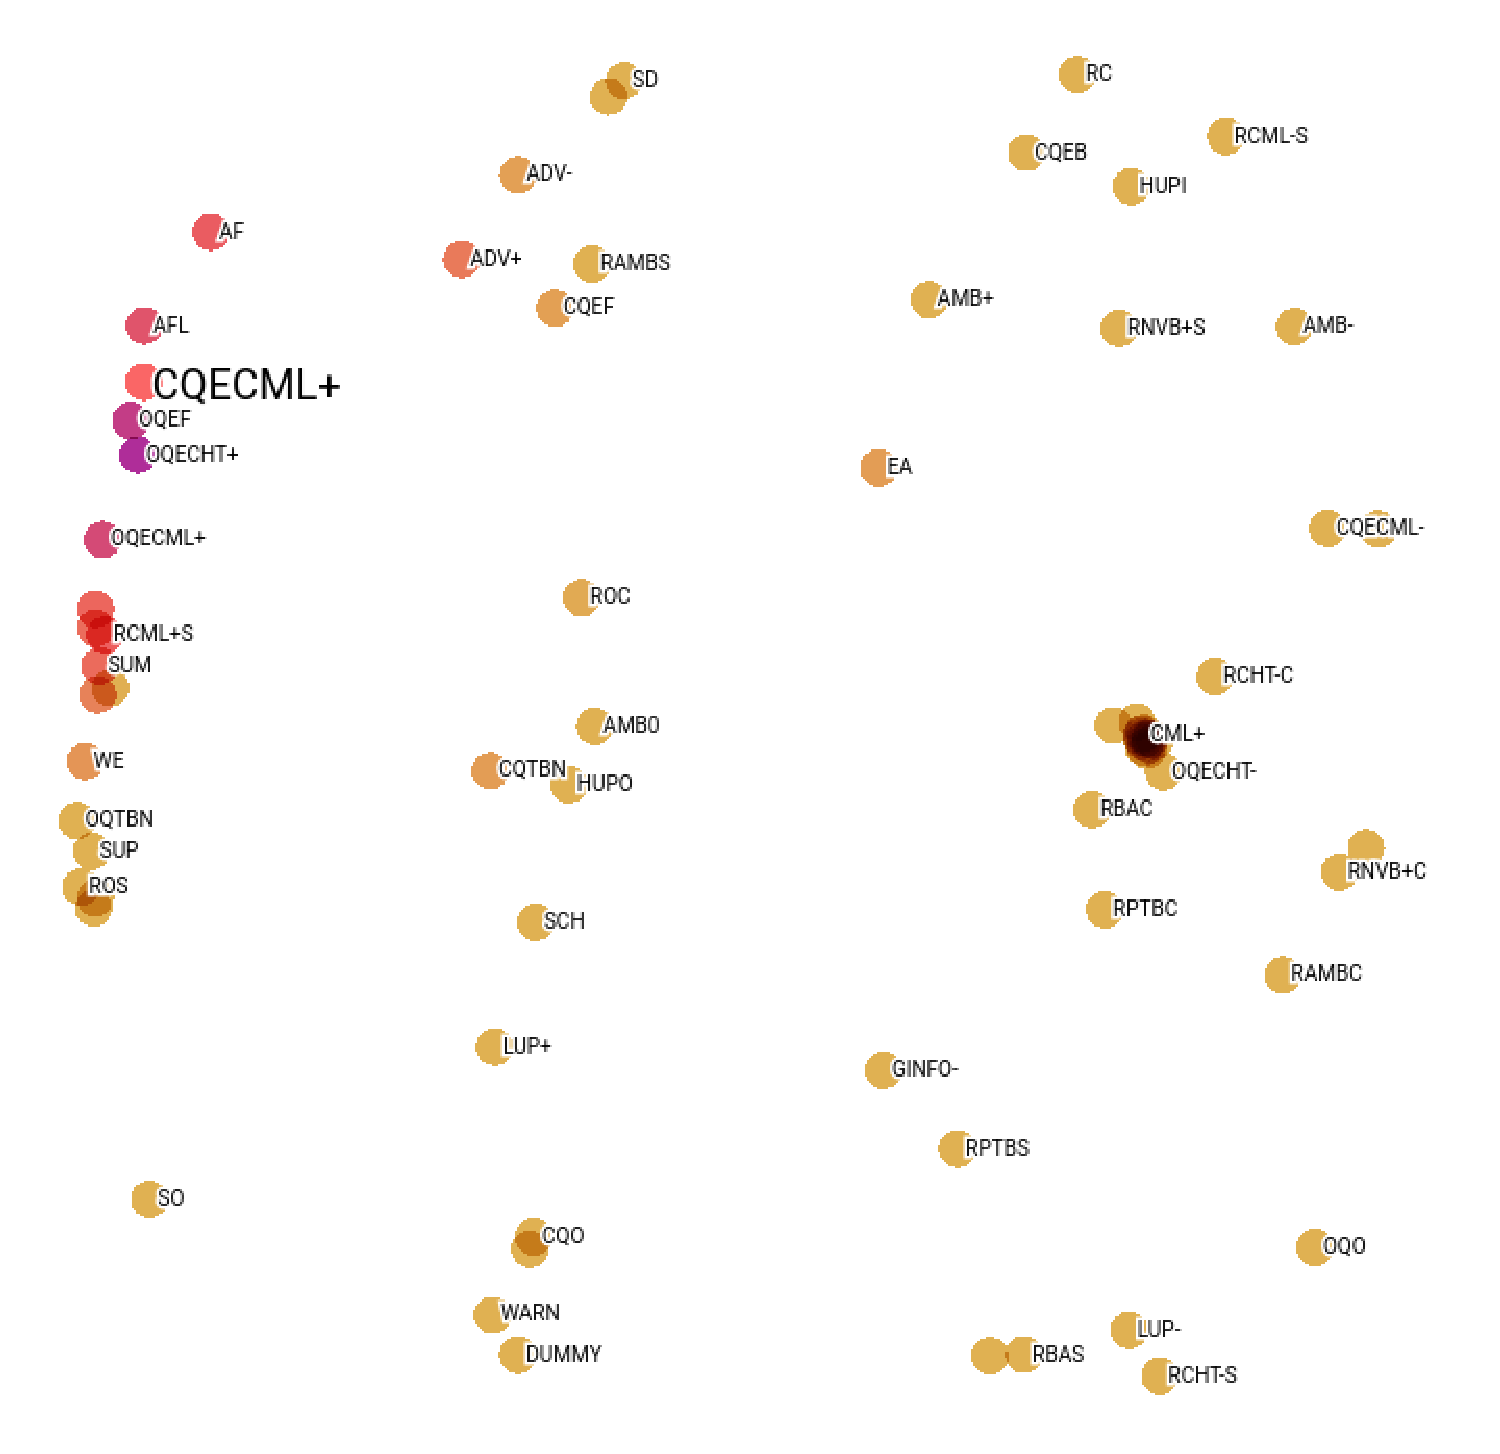
\includegraphics[width=0.50\textwidth]{figures/code_embed.eps}
    \caption{\textbf{T-SNE diagram of behavior codes drawn after 4000 steps with perplexity 30}.}
    \label{fig:code_embedding}
\end{figure}

\textbf {Recurrent Neural Network (RNN)} is a type of Neural Network, which can send feedback from the current hidden state to the hidden state of the next time step. That RNN can capture long-term dependencies for predicting the future events is its main advantage of RNN over feedforward Neural Network, MC, and HMM. The capability of remembering past event is very useful in motivational interviews where a behavior observed at some points in the interview is very informative for the future behaviors that will be observed. However, it was observed that RNN fails to capture long-term dependencies due to vanishing gradient problem \cite{bengio1993problem}. In order to mitigate this problem, Hochreiter et al.\cite{hochreiter1997long} proposed a special kind of RNN called Long Short Term Memory networks or simply LSTM. Later, the model was enhanced by including forget gates and the tanh activation function \cite{graves2013speech}. There are several variants of LSTM model, where a dramatic variation on the LSTM is the Gated Recurrent Unit\cite{cho2014properties} or simply GRU. GRUs are simpler than LSTM units and experimentally outperform than other models in many cases. We reiterate the mathematical formulation of GRU defined by Chung et al.\cite{chung2014empirical} as follows (Eq.~\ref{eq:firstgru}~to~\ref{eq:lastgru}):
\begin{equation}
z_t = \sigma(W_zx_t + U_zh_{t-1} + b_z)
\label{eq:firstgru}
\end{equation}
\begin{equation}
r_t = \sigma(W_rx_t + U_rh_{t-1} + b_r)
\end{equation}
\begin{equation}
\tilde h_t = tanh(W_hx_t + r_t \odot U_hh_{t-1} + b_h) 
\end{equation}
\begin{equation}
h_t = z_t \odot h_{t-1} + (1-z_t) \odot \tilde h_t
\label{eq:lastgru}
\end{equation}  
\begin{equation}
total\ loss = \alpha \cdot \frac{1}{T}\sum_{t=1}^T loss(\bar y^{(t)},y^{(t)}) + (1 - \alpha) \cdot loss(\bar y^{(T)},y^{(T)})
\label{eq:loss}
\end{equation}  
\begin{figure}[!htb]
    \centering
    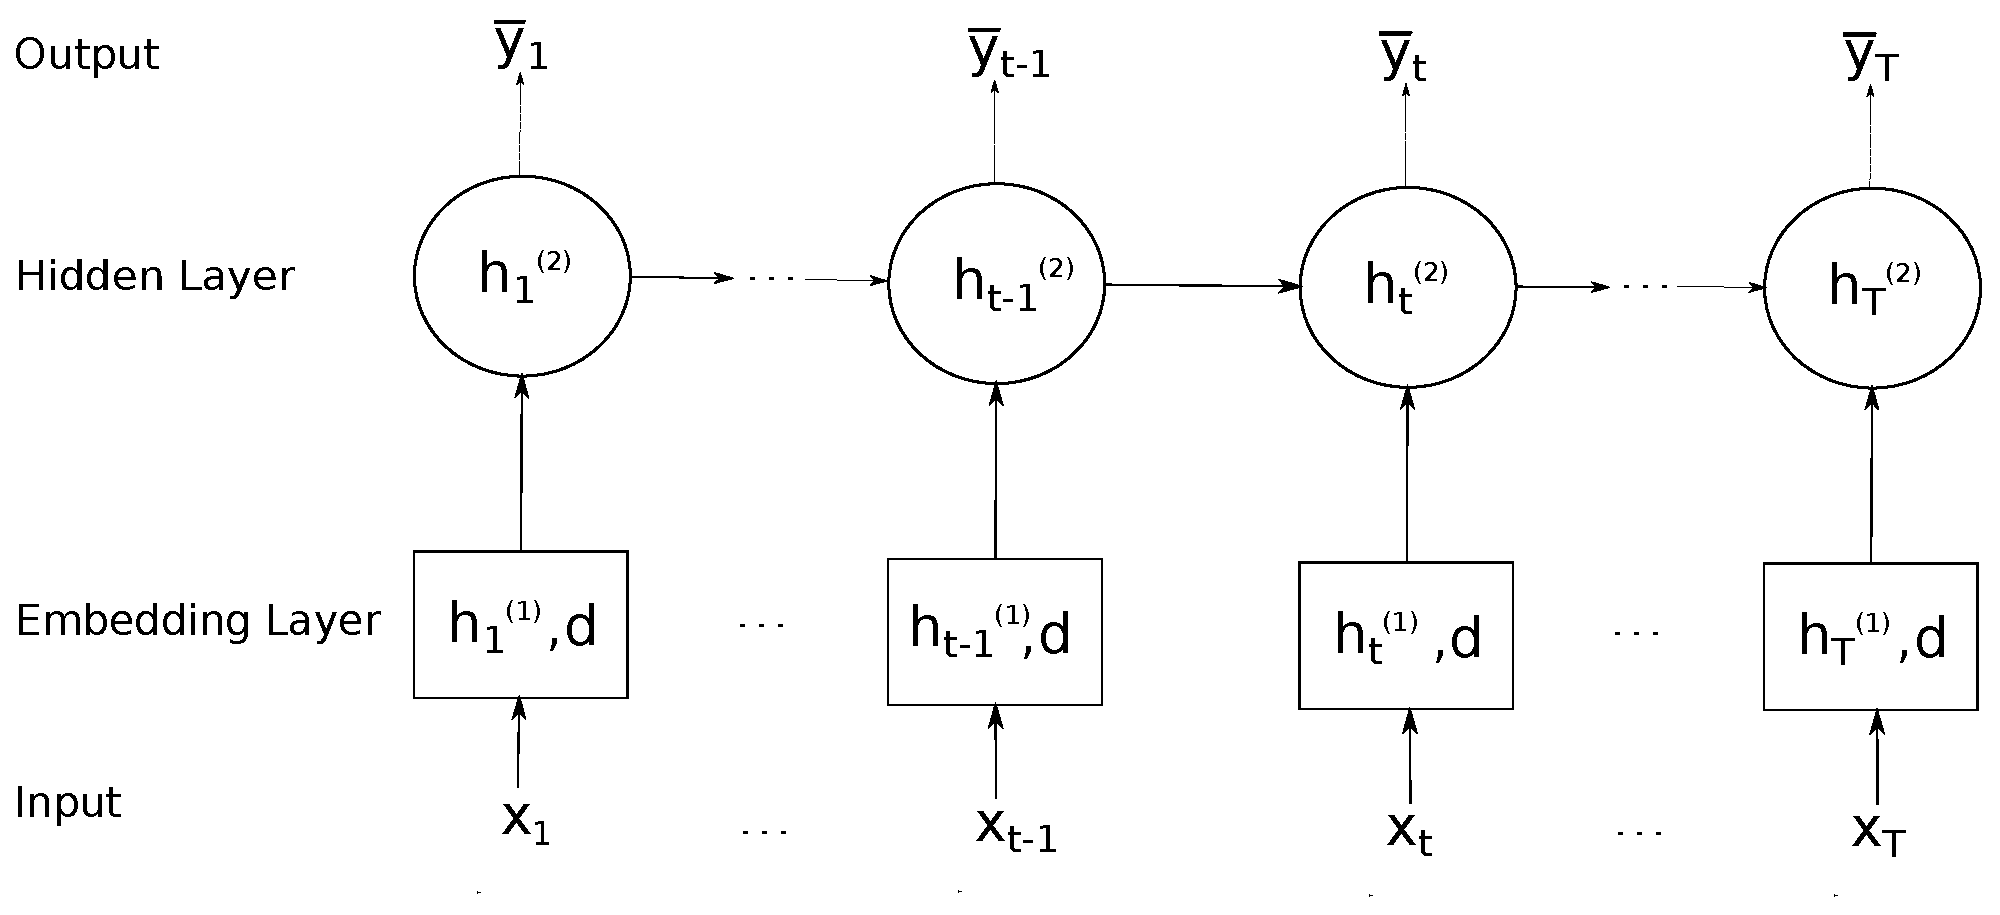
\includegraphics[width=0.70\textwidth]{figures/rnn.eps}
    \caption{\textbf{Proposed RNN model with target replication (TR)}.}
    \label{fig:rnn-model}
\end{figure}
The architecture of the proposed Recurrent Neural Network is shown in Figure~\ref{fig:rnn-model}. We used one hidden layer of 15 LSTM or GRU nodes after embedding the given MYSCOPE codes from the input sequence. Then, we applied a softmax layer at each time-step for predicting the target which is the label of the entire sequence (successful or unsuccessful). This target replication (TR) strategy was used in several studies \cite{lipton2015learning, choi2016doctor} after introduced by Lee et al.\cite{lee2015deeply} in 2015 for convolutional neural networks. As it can be seen from equation~(\ref{eq:loss}), total loss of our prediction models is the combination of final loss and the mean of the losses over all sequence steps, where T is the total number of sequence step, $\bar y^{(t)}$ is the output at step t, and $\alpha\ \epsilon\ [0, 1]$ is a hyperparameter that determines the relative importance of intermediate outputs. Experimentally, it was determined that best performance achieved when we use  $\alpha=0.5$. Our model also contains several other hyperparameters such as embedding dimension, number of hidden units, learning rate, batch size, etc., which were determined by the validation set. We implemented our models in Tensorflow with Adam optimizer and early stopping based on the validation loss. Experimentally, we observed that our model converges to optimal after 100 epoch and have no effect of dropout and regularization. The code for all models is publicly available at https://github.com/teanalab/myscope-sequential-analysis.   
  
\subsection*{\textit{Evaluation metrics}}
Performance of the proposed method was evaluated in terms of precision, recall, and F-measure using 10 folds cross-validation and weighted macro-averaging of these metrics over the folds. However, LSTM and GRU are trained on 80\% of the data and validated on 10\%. The remaining 10\% of the data is used as a test set for reporting the performance of the model. A true positive (TP) was counted when the method correctly classified a sequence into its actual class; a false positive (FP) was counted for a class when the method incorrectly classified a sequence into that class; a false negative (FN) for an actual class of sequence was counted when the method incorrectly classified the sequence into other class. The Precision of a class was defined as the ratio of the numbers of correctly classified sequences and all sequences identified as belonging to that particular class by the classifier (i.e Precision = TP / (TP + FP)). Recall of a class was defined as the ratio between the numbers of correctly classified sequences and all sequences of that particular class in the gold standard (i.e. Recall = TP / (TP + FN)). F-measure is computed as the harmonic mean of precision and recall (i.e. 2 x Precision x Recall / (Precision + Recall)). 

\section*{Results}
Experimental evaluation of the proposed method is conducted on both under and over-sampled sequences. Predictive performance summary of the proposed methods on under and over-sampled sequences is presented in Table~\ref{tab:result_under_over_sampled}.\\ 
\begin{table}[h]
\centering
\caption{Performance of MC, HMM, and RNN for predicting the success of under and over-sampled patient-provider communication sequences. The highest value for each performance metric is highlighted in bold.}
\label{tab:result_under_over_sampled}
  \begin{tabular}{|l|l|l|l|l|l|l|}
  \hline
   \multirow{2}{*}{\textbf{Method}} & \multicolumn{3}{|c|}{\textbf{Undersampling}} & \multicolumn{3}{|c|}{\textbf{Oversampling}} \\\cline{2-7}
   & \textbf{Precision}  & \textbf{Recall} & \textbf{F1-Score} & \textbf{Precision}  & \textbf{Recall} & \textbf{F1-Score}\\ \hline    
    
 Markov Chain $1^{st}$ Order & 0.7060 & 0.7044 & 0.7038 & 0.7932 & 0.7799 & 0.7775 \\ \hline
 Markov Chain $2^{nd}$ Order & 0.6395 & 0.6385 & 0.6379 & 0.7111 & 0.7029 & 0.7000\\ \hline
 Hidden Markov Model & 0.6244 & 0.6143 & 0.6067 & 0.7775 & 0.7567 & 0.7520\\ \hline
 LSTM RNN & 0.8672 & 0.8626 & 0.8622 & 0.8411 & 0.8372 & 0.8368\\ \hline
 LSTM RNN - TR & \textbf{0.8733} & \textbf{0.8681} & \textbf{0.8677} & \textbf{0.8424} & \textbf{0.8385} & \textbf{0.8381}\\ \hline
 GRU RNN & 0.8674 & 0.8648 & 0.8646 & 0.8379 & 0.8342 & 0.8337\\ \hline
 GRU RNN - TR & 0.8705 & 0.8676 & 0.8673 & 0.8412 & 0.8377 & 0.8373\\ \hline 
  \end{tabular}
\end{table}  

\subsection*{\textit{Predictive performance for under-sampled PPC code sequences}}
We applied small learning rate (0.00005) and batch size (8) with early stopping strategy for training deep learning models when the under-sampled dataset is used. Five major conclusions can be drawn from the results in Table~\ref{tab:result_under_over_sampled}. First, recurrent neural networks outperform over probabilistic models and achieved 16.39\%-26.1\% higher F1-score. Second, LSTM with target replication has the best performance over all other RNN methods, and achieved F1-score 0.8677 with precision 0.8733 and recall 0.8681. Third, target replication strategy improves the performance of GRU and LSTM, while conventional GRU shows better performance than traditional LSTM. Fourth, among probabilistic models, the MC-based method generally outperforms HMM across all metrics for under-sampled sequences. Fifth, it follows that second-order MC have lower precision, recall, and F-measure than first-order MC. In particular, precision, recall and F-measure decrease by 9.42\%, 9.36\% and 9.36\%, when going from first to second-order models.

\subsection*{\textit{Predictive performance for over-sampled PPC code sequences}}
Similar to the under-sampled dataset, early stopping strategy was also employed for the over-sampled dataset. For over-sampled data, RNN models were trained with learning rate 0.00010 and batch size 55. Experimental results indicate that HMM had better performance than second-order MC, achieving 9.34\%, 7.65\%, and 7.43\% higher precision, recall, and F-measure, while HMM still has 1.98\%, 2.97\%, and 3.28\% lower precision, recall, and F-measure than first-order Markov chain. Similar to under-sampled sequences, target replication improves the performance of RNN models, and LSTM with target replication has the highest F1-score among all models. However, the predictive performance of recurrent neural networks decreases in over-sampled sequences although the performance of probabilistic models increases. We also observed that all models have the largest value in precision compared to other performance metrics.

\begin{table}[h]
\centering
\caption{Most likely communication sequences in successful and unsuccessful motivational interviews.}
\label{tab:common_patterns}
  \begin{tabular}{|l|l|}
  \hline
   \textbf{Type} & \textbf{Most likely communication sequences} \\ \hline      
successful & GINFO+: General information, positive $\rightarrow $ LUP+: Low uptake, positive $\rightarrow $ OQTBN: \\ 
& Open-ended question, target behavior neutral \\\hline
successful & SS: Structure session $\rightarrow $ GINFO+: General information, positive $\rightarrow $ CQECHT+: Closed-ended \\
& question, elicit change talk positive\\\hline
successful & SO: Statement, other $\rightarrow $ LUP+: Low uptake, positive $\rightarrow $ AF: Affirm $\rightarrow $ HUPW: High uptake, \\
& weight $\rightarrow $ OQECML+: Open-ended question, elicit commitment language positive. \\\hline
unsuccessful & ADV+: Advise, positive $\rightarrow $ AMB-: Ambivalence negative $\rightarrow $ OQECHT-: Open-ended \\
& question, elicit change talk negative\\\hline
unsuccessful & CQECHT+: Open-ended question, elicit change talk positive $\rightarrow $ RCHT-S: Reflect, change talk \\
& negative $\rightarrow $ OQECHT-: Open-ended question, elicit change talk negative \\\hline
unsuccessful & SUP: Support $\rightarrow $ AF: Affirm $\rightarrow $ CQTBN: Closed-ended question, target behavior neutral \\
& $\rightarrow $ OQECHT-: Open-ended question, elicit change talk negative $\rightarrow $ AMB-: Ambivalence negative\\\hline
  \end{tabular}
\end{table} 

\subsection*{\textit{Most likely communication sequences}}
Table~\ref{tab:common_patterns} provides examples of typical patient-provider communication sequences that frequently appear in successful and unsuccessful motivational interviews. In successful sequences, we observed the provision of information using patient-centered communication (GINFO+) and structure session which is the counselor either explaining the therapeutic agenda or attempting to transition to a new topic or session content (SS). Sometimes, counselor acknowledged the clients' communication or an off topic comment (SO). We also observed that the affirm and OQECML+ are consistent with MI theory as an effect for eliciting positive change talk or commitment language. For unsuccessful sequences, It can be seen that providing advice using non-patient centered strategies (ADV-) leads to the ambivalence that is weighted against change (AMB-) which is heading in the wrong direction therapeutically. Questions phased to elicit negative change talk or commitment language leads to CHT- or CML-, which is consistent with the manual coding approach or analysis, or AMB-.
%It can be seen that most successful sequence starts with a summary of the discussion or structured statement. After that, if adolescents express positive change talk, the counselor immediately reflects on that to reinforce adolescent's intrinsic motivation about behavior change. On the other hand, asking open- or closed-ended questions with eliciting negative change talk can lead to negative change talk, even in the cases when adolescents were showing a positive tendency in their previous communication. This observation can be explained by adolescents quickly confused when reiterating negative information that undermines their motivation. Analyzing such cases will allow the counselors to determine the negative information that can be discussed during the interviews.

\section*{Discussion}
By analyzing the experimental results of different communication sequence outcome prediction schemes proposed in this paper, we arrived at the following conclusions. First, the overall predictive performance of RNN models is substantially better than probabilistic models. In particular, the RNN-based method achieves near-human accuracy for predicting the label of motivational interviews. This indicates that RNN is able to capture the structure of discourse in motivational interviews by preserving long-term dependencies among the behavior codes, which reflect the overall progression of the interviews. This provides evidence that the RNN is able to successfully replicate human cognitive processes to integrate previous information when formulating higher level thinking. In addition to that, word-embedding allows to reduce the dimensionality of codes in PPC sequences and consequently improve both precision and recall of the prediction method. 

Second, using target replication to compute the losses at each time step results in better performance for all configurations of the proposed RNN method. This indicates that mean of the losses over all steps emphasize the dependencies between the pairs of patient and provider codes, which results in more accurate estimates of the model parameters. Better estimates of parameters in RNN models of motivational interviews are propagated to the next step based on the relative importance of intermediate output, where they are aggregated into predictions for the entire sequence. This allows achieving an improvement in the prediction accuracy of the method. 

Third, using first-order Markov model results in better prediction accuracy compared to higher-order Markov models. Because the number of states in higher-order Markov models grows exponentially with their order. Therefore, accurate estimation of transition probabilities requires much larger training set. Using smaller datasets such as under-sampled dataset will result in a sparsity problem, when many transitions are either not observed in the training set at all or observed only a few times, leading to missing or potentially inaccurate probability estimates. Obtaining large training sets cannot be easily accomplished in many domains, including motivational interviewing. In this study, we found out that using first-order Markov models is a reasonable trade-off between efficiency and accuracy.  

Fourth, similar to traditional Markov model, HMM achieve a dramatic improvement in the prediction accuracy when larger training set is used. This indicates that sufficient training data is required to estimate optimal hyperparameters such as a number of hidden states, initial state distribution, transition probabilities, and emission probabilities.   
 
Fifth, the proposed method can be used to identify the most effective communication strategies at eliciting a particular type of behavioral response. Awareness of these strategies by researchers can significantly decrease the time and effort required to develop effective interventions to address many public health conditions, such as childhood obesity, and tailor these interventions to particular patient cohorts. Awareness of these strategies by the counselors can lead to a greater success rate of motivational interviews.     
 
\section*{Conclusion}
In this paper, we proposed Recurrent Neural Networks with two baseline methods Markov Chain and Hidden Markov Model for predicting the success of motivational interviews. We found out that individual patient-provider communication exchanges are highly indicative of the overall progression and future trajectory of clinical interviews and can be used to predict their overall success. Our proposed method can facilitate motivational interviewing researchers in establishing causal relationships between different communication strategies and the desired behavioral outcomes during the interviews without resource-intensive manual qualitative analysis of interview transcripts. Our proposed method can also help to identify most likely sequences that are common to successful and unsuccessful motivational interviews, which can also directly inform clinical practice. This work also has broad implications for qualitative public health research by providing a formal theoretically-grounded computational mechanism to facilitate the development of effective behavioral interventions.

\section*{Acknowledgments}
This study was supported by a grant from the National Institutes of Health, NIDDK R21DK108071, Carcone and Kotov, MPIs. We would like to thank the student assistants in the Department of Family Medicine and Public Health Sciences at Wayne State University School of Medicine for their help in developing the training data set by manually annotating the data set using the MYSCOPE codebook. 
%\pagebreak

\bibliographystyle{vancouver}
\bibliography{references}

\end{document}